\documentclass[12pt,utf8]{beamer}

%-----PARAMETERS-----

%Wichtige Standard Pakete!
%\usepackage[german]{babel}
\usepackage{ngerman}
\usepackage{xcolor}
\usepackage{graphicx}
\usepackage{tikz}

%Für den Header notwendig!
%\usepackage[percent]{overpic}

\usepackage{hyperref} % für korrekte Links

%Einbinden des Themes
\input{Latex_Template/beamerthemeFOSSAG.sty}

%Titelangaben
\title{Free my Android - Step 1}
\subtitle{Wie man sein Smartphone fit hält}

\author{Christoph Parnitzke}
\institute[FOSS AG]{\textbf{F}ree and \textbf{O}pen \textbf{S}ource \textbf{S}oftware \textbf{AG}}

\date{25. Juni 2017}


%-----IMPLEMENTATION-----
\begin{document}

\begin{frame}
	\titlepage
\end{frame}

\begin{frame}{Inhaltsverzeichnis}
	\tableofcontents
	\note{Derivate entsprechen Distributionen bei Linux}
\end{frame}

\section{Android - ein Werdegang}

\begin{frame}{Inhaltsverzeichnis}
	\tableofcontents[currentsection, hideallsubsections]
\end{frame}


\begin{frame}{Android - Ein Werdegang}
	\begin{itemize}[<+->]
		\item[2003 -] Android, gegründet von Andy Rubin
		\begin{itemize}	
			\item<1-> Unternehmen zur Entwicklung von Mobilsoftware \\(urspr. für Digitalkameras)
		\end{itemize}
		\item[2005 -] Übernahme durch Google
		\item[2007 -] Ankündigung eines neuen Mobiltelefon-OS der Open Handset Alliance
		\item[2008 -] Veröffentlichung des ersten Android OS
		\item[2015 -] Google trennt Sicherheitsupdates von Android-Upgrades
	\end{itemize}
\end{frame}

\begin{frame}{Das Nexus - Der direkte Draht zu Android}
	\begin{itemize}[<+->]
		\item Die Nexus Serie wurde zwischen 2010 und 2016 von Hardwarepartnern hergestellt
		\item Sie erhielt immer die topaktuelle Software aus dem Hause Google
		\item Nexus wurde 2016 durch Pixel abgelöst.
	\end{itemize}
\end{frame}

\begin{frame}{Der Erfolg eines freien Betriebssystems}
	\begin{figure}
		
\includegraphics[scale=0.35]{resources/att.jpg}
	\end{figure}
	\begin{itemize}[<+->]
		\item Freiheit des Codes trug zur Fehlersuche und Verbreitung bei
		\item Offener Code ermöglichte Entwicklercommunities wie XDA-Developers
	\end{itemize}
\end{frame}

\begin{frame}{Der Erfolg eines freien Betriebssystems}
	\begin{itemize}[<+->]
		\item Das kostenlosen und freie Android wurde schnell beliebt
		\item 2016 war das OS zu 87,5\% auf dem Markt vertreten
		\item Dabei ist das System stark fragmentiert
		\begin{itemize}
			\item Viele Hersteller verbreiten eigene Portierungen des Systems
			\item Viele CustomROMs von bspw. XDA-Developers fragmentieren zusätzlich 
		\end{itemize}
	\end{itemize}
\end{frame}

%\\end of section "Prologue"

\section{Das Android-Betriebssystem}

\begin{frame}{Inhaltsverzeichnis}
	\tableofcontents[currentsection, hideallsubsections]
\end{frame}

\begin{frame}{Android ist Hardware-Spezifisch}
	\begin{itemize}[<+->]
		\item Jedes System muss auf die gegebene Hardware des Gerätes angepasst werden
		\begin{itemize}
			\item Verhindert einen übergroßen Kernel
			\item Spart Speicher
			\item Erhöht Performance
		\end{itemize}
		\item Das verkompliziert das Anpassen von CustomROMs da die jeweiligen Geräte zum Testen benötigt werden
	\end{itemize}
\end{frame}

\begin{frame}{Struktur der Software}
	\begin{itemize}[<+->]
		\item Android teilt sich in folgende Partitionen:
		\begin{itemize}
			\item Bootloader 
			\item Recovery
			\item System
			\item Data
			\item SDCard / ExtSDCard
			\item Cache
		\end{itemize}
		\item Dazu kommen kleinere Partitionen welche weitere Systemfunktionen garantieren.
	\end{itemize}
	\pnote{ Bootloader: Lädt den Kernel und das schlussendliche System}
	\pnote{ Recovery: Ist ein "Rettungssystem", welches erweiterte Funktionen auf dem Gerät zur Verfügung stellen kann. (Backups, zusätzliche Pakete installieren, etc.)}
	\pnote{ System: Das Betriebssystem an sich}
	\pnote{ Data: Benutzerdatenpartition; Hier werden Kontakte, Nachrichten, Dauerhafte Appdaten und mehr gelagert}
	\pnote{ SDCard: Zusätzlicher Speicher der dem Nutzer frei zur Verfügung steht. Hier werden heruntergeladene Dateien, Musik, Bilder und Videos und weiteres gespeichert.}
	\pnote{ Cache: Partition zum Speichern temporärer Daten. Kann bedenkenlos geleert werden.}
\end{frame}

%\\end of section "Android_the_OS"

\section{Android-Derivate}

\begin{frame}{Inhaltsverzeichnis}
	\tableofcontents[currentsection, hideallsubsections]
\end{frame}

\begin{frame}{Android-Derivate}
\begin{columns}
	\begin{column}{0.5\textwidth}
		\begin{figure}
			
\includegraphics[width=0.9\textwidth]{resources/Lineage_OS_Logo.png}
			%https://de.wikipedia.org/wiki/Linux_Mint#/media/File:Linux_Mint_logo_and_wordmark.svg
		\end{figure}
		
		\begin{figure}
			
\includegraphics[width=0.8\textwidth]{resources/aokp-logo-large.png}
			%https://de.wikipedia.org/wiki/OpenSUSE#/media/File:OpenSUSE_Logo.svg
		\end{figure}
		
	\end{column}
	\begin{column}{0.5\textwidth}
		
		\begin{figure}
			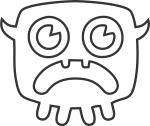
\includegraphics[scale=2]{resources/PA-Head.png}
			%https://de.wikipedia.org/wiki/Ubuntu#/media/File:Ubuntu_logo.svg
		\end{figure}
		
		\begin{figure}
			
\includegraphics[scale=0.15]{resources/Replicant_logo_alpha.png}
			%https://de.wikipedia.org/wiki/Fedora_%28Linux-Distribution%29#/media/File:Fedora_logo_and_wordmark.svg
		\end{figure}
		
	\end{column}
\end{columns}
\end{frame}

\begin{frame}{LineageOS}
	\begin{figure}
		
\includegraphics[scale=0.25]{resources/Lineage_OS_Logo.png}
	\end{figure}
	\begin{itemize}[<+->]
		\item Erwuchs Weihnachten 2016 aus dem eingestellten CyanogenMod (\textbf{CM})
		\item CM war bis zu diesem Zeitpunkt das am weitesten verbreitete und unterstützte CustomROM
	\end{itemize}
\end{frame}

\begin{frame}{LineageOS}
	\begin{itemize}[<+->]
		\item LineageOS wird nun ausschließlich von der Community und einigen Entwicklern auf GitHub entwickelt
		\item Es unterstützt bis heute die meisten Geräte und bringt viele zusätzliche Features
		\item Daher werden wir nun exemplarisch ein LineageOS How-To-Flash für ein OnePlus One durchführen
	\end{itemize}
\end{frame}

%\\end of section "Derivates"

\section{Werkzeuge}

\begin{frame}{Inhaltsverzeichnis}
\tableofcontents[currentsection, hideallsubsections]
\end{frame}

\begin{frame}{Das Flashen - ADB}
	\begin{itemize}[<+->]
		\item Die \textbf{A}ndroid \textbf{D}ebug \textbf{B}ridge ist ein wichtiges Werkzeug
		\item Sie ermöglicht das Arbeiten und Kommunizieren mit dem Android System über eine USB oder WLAN Verbindung
		\item Mit ihr wird es möglich Dateien von und zum Rechner zu verschieben.
		\item Die \textbf{ADB} wird insbesondere zum Übertragen neuer CustomROMs verwendet, es gibt aber auch weitere Möglichkeiten.
		\begin{itemize}[<+->]
			\item Übertragen und Installieren von Apps mit dem Rechner
			\item Verwenden einer Shell vom Rechner aus
		\end{itemize}
	\end{itemize}
\end{frame}

\begin{frame}{Das Flashen - Fastboot}
	\begin{itemize}[<+->]
		\item Das \textbf{Fastboot}-Tool arbeitet eine Ebene tiefer im System
		\item Statt mit dem laufenden Android OS zu kommunizieren arbeitet es direkt auf der Firmware des Geräts
		\item Fastboot ermöglicht bei vielen Geräten das Entsperren des Bootloader-Sektors
		\begin{itemize}[<+->]
			\item Diese Funktion wird zum Flashen von Android-Derivaten benötigt
		\end{itemize}
		\item Außerdem können mit Fastboot direkt Images geflashed werden
	\end{itemize}
\end{frame}

\begin{frame}{Das Flashen - Mehr braucht es nicht?}
	\begin{itemize}[<+->]
		\item Die zuvor vorgestellten Tools reichen theoretisch zum Aufspielen alternativer Software aus
		\item Angepasste Android Versionen haben aber unter Umständen andere Schutzmechanismen
		\note{ Leider haben in der Praxis viele Hersteller eigene Wege entwickelt ihre Bootloader vor Zugriff zu schützen oder ein Aufspielen anderer Software zu limitieren }
		\item Daher braucht man je nach Gerät andere Software
		\item Wir gehen zusätzlich nur auf Samsung ein
		\note{ Der Verbreitung der Marke geschuldet gehen }
	\end{itemize}
\end{frame}

\begin{frame}{Das Flashen - Heimdall/Odin}
	\begin{itemize}[<+->]
		\item Heimdall und Odin sind für Samsung-Geräte erstellte Software
		\item Sie ersetzen Fastboot in ihrer Funktion
		\item Während Odin ein sog. Leak ist, wird Heimdall frei entwickelt.
	\end{itemize}
\end{frame}


%\\end of section "Utilities"

\section{How To Flash}

\begin{frame}{Inhaltsverzeichnis}
\tableofcontents[currentsection, hideallsubsections]
\end{frame}

\begin{frame}{Das Flashen}
	\begin{figure}
		
\includegraphics[scale=0.2]{resources/OSHA-Watch-Your-Step-Sign-OBE-6440_1000.jpg}
	\end{figure}
	\begin{itemize}[<+->]
		\item Was auch immer ihr ab hier nachmacht: Seid vorsichtig!
		\item Es gibt viele Menschen mit gefährlichem Halbwissen
		\item Und wie immer gilt: Backups, Backups, Backups!
	\end{itemize}
	\pnote{ Datenverlust ist möglich }
\end{frame}

%\\end of section "How_To_Flash"

%\section{Fazit}

%\input{Epilogue.tex}

%\\end of section "Epilogue"

\end{document}
